\documentclass{beamer}
%\usepackage{caption}
%
\usepackage{subcaption}
\usepackage{../arbenson-math}
\usepackage{wasysym}

\newcommand{\A}{\mathcal{A}}
\newcommand{\B}{\mathcal{B}}

\usetheme{boxes}
\usecolortheme{seahorse}

\setbeamertemplate{frametitle}
{
    \nointerlineskip
    \begin{beamercolorbox}[sep=0.3cm,ht=1.8em,wd=\paperwidth]{frametitle}
        \vbox{}\vskip-2ex%
        \strut\insertframetitle\strut \hfill \insertframenumber
        \vskip-0.8ex%
    \end{beamercolorbox}
}

\AtBeginSection[]
{
  \begin{frame}<beamer>
    \frametitle{\insertsection}
    \tableofcontents[currentsection]
  \end{frame}
}

\titlegraphic{}

\title{Silent error resilience in numerical time-stepping schemes}
\author{
Austin Benson \\
Institute for Computational and Mathematical Engineering \\
Stanford University \\
HP Labs
\vspace{0.1in}
Sven Schmit (ICME) and Rob Schreiber (HP Labs)
\vspace*{-1cm}
}
SIAM PP 2014
\date{February 19, 2014}
\begin{document}
\maketitle

%
\begin{frame}
\frametitle{Illustrative example}

\begin{figure}
  \centering
  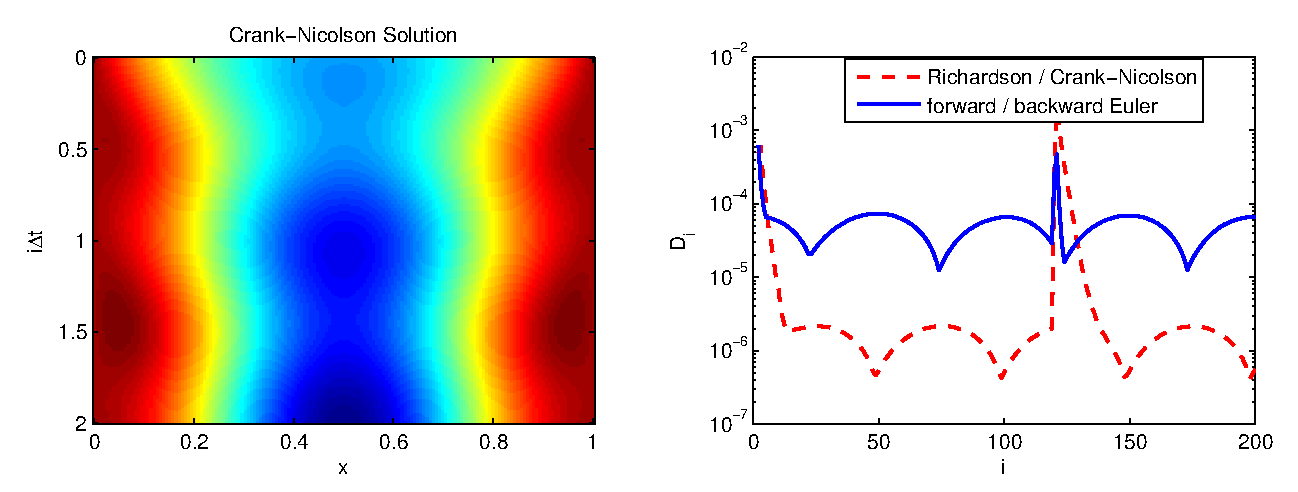
\includegraphics[scale=0.7]{img/heat_soln_diffs1.eps}
\end{figure}

\delta_x = \frac{1}{160}, \delta_t = \frac{1}{100}

\begin{align}
& u_t = \frac{1}{100}u_{xx} + 0.1\left(\sin(2\pi t) + \cos(2\pi x)\right) \nonumber \\
& t \in [0, 2], x \in [0, 1]
& u(x, 0) = x(x-1) \nonumber \\
\end{align}


%
\begin{frame}
\frametitle{Main idea}

\begin{figure}
  \centering
  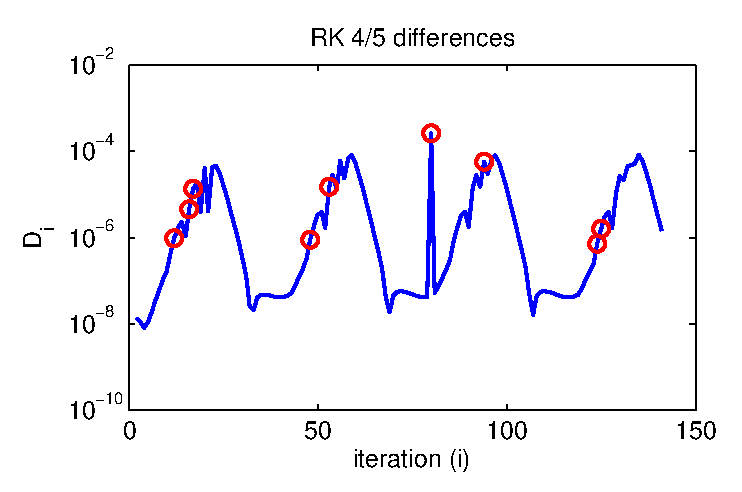
\includegraphics[scale=0.7]{img/vdp2_rk.eps}
\end{figure}

\begin{itemize}
\setlength{\itemsep}{0.15in}
\item{Base method $\B$ generates $B_1, B_2, \ldots$}
\pause
\item{Auxiliary method $\A$ ``checks'' with $A_1, A_2, \ldots$}
\pause
\item{$D_i = ||B_i - A_i||$ abnormal $\to$ possible error}
\end{itemize}
\end{frame}

%
\begin{frame}
\frametitle{What are these things?}

\begin{figure}
  \centering
  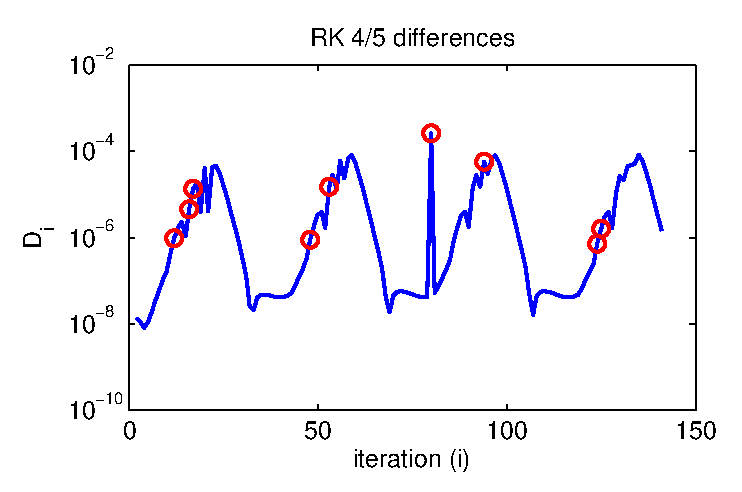
\includegraphics[scale=0.7]{img/vdp2_rk.eps}
\end{figure}

\begin{itemize}
\setlength{\itemsep}{0.15in}
\item{Base method $\B$: higher-order scheme (Runge-Kutta 5)}
\pause
\item{Auxiliary method $\A$ ``checks'': lower-order scheme (Runge-Kutta 4)}
\pause
\item{Want $\A$ needs to be cheap: embedded pairs}
\end{itemize}
\end{frame}

[Fehlberg, 1969] \\
[Dormand and Prince, 1980]

%
\begin{frame}
\frametitle{Lots of these schemes}

\begin{itemize}
\item Backward / Forward Euler, Richardson scheme
\item Runge-Kutta 4/5, 2/3
\item Adams-Bashforth 4/5, 2/3
\item Explicit check on implicit scheme
\item Extrapolation
\end{itemize}

\begin{center}
Auxiliary method $\A$ re-uses data (and communication) from base method $\B$
\end{center}

\end{frame}

%
\begin{frame}
\frametitle{Detecting errors}

\begin{figure}
  \centering
  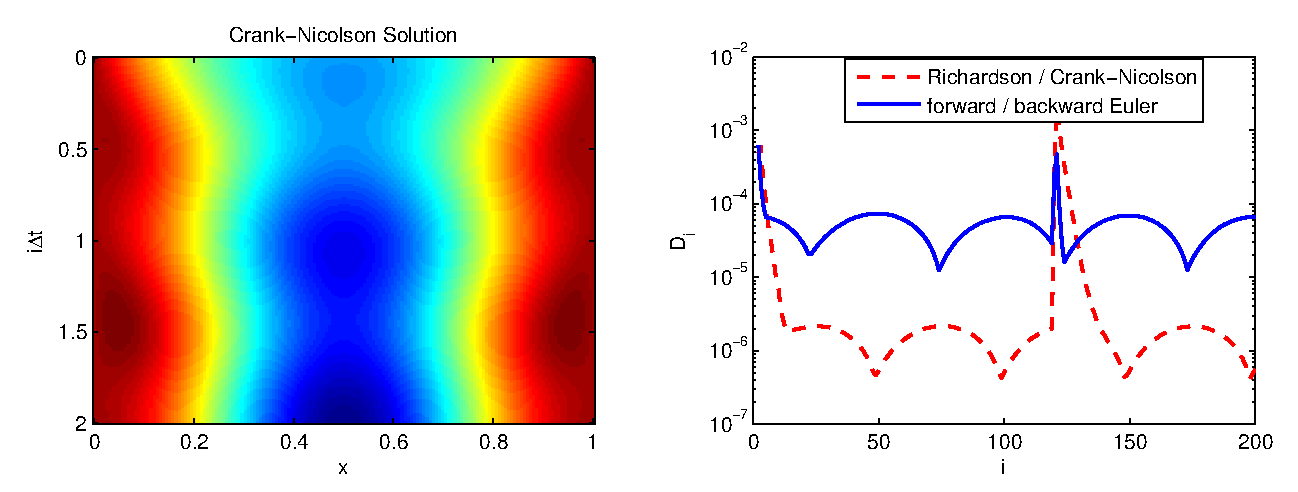
\includegraphics[scale=0.7]{img/heat_soln_diffs1.eps}
\end{figure}

\begin{itemize}
\item Sequence $D_i = \| B_i - A_i \|$: differences between true scheme and checking scheme
\item Look at jumps
\item Look at variance
\end{itemize}

\end{frame}

\begin{frame}
\frametitle{Detecting errors}

\begin{figure}
  \centering
  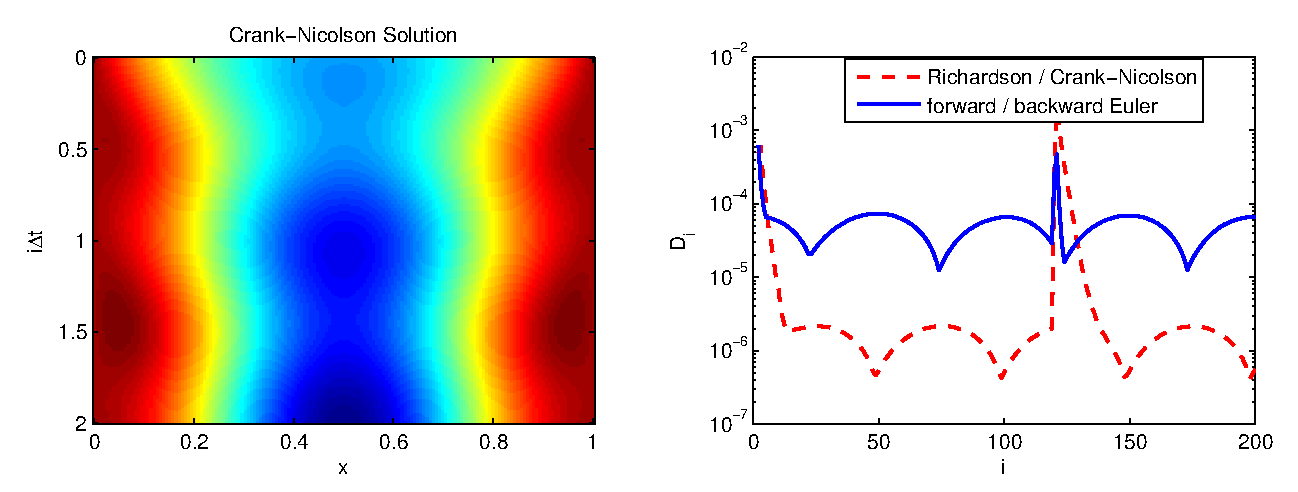
\includegraphics[scale=0.7]{img/heat_soln_diffs1.eps}
\end{figure}

% TODO: Put in error detection algorithm here

\end{frame}


%
\begin{frame}
\frametitle{Error impact}

\begin{itemize}
\item $B_n$ and $A_n$ are the outputs of $\B$ and $\A$ when \emph{a fault is injected}
\item $\hat{B}_n$ and $\hat{A}_n$ are the outputs of $\B$ and $\A$ when \emph{no fault is injected}
\end{itemize}

\begin{center}
Local truncation error-normalized error:
\[
L_n = \frac{\| B_n - \hat{B}_n \|}{\| \hat{B}_n - \hat{A}_n \|} = \frac{\text{Difference caused by error}}{\text{Estimate of local truncation error}}
\]
\end{center}

\end{frame}

%
\begin{frame}
\frametitle{Detecting errors in Adams-Bashforth}

\[
u^{\prime\prime}(t) - b(1 - u(t)^2)u^{\prime}(t) + u(t) = 0
\]
\[
u(0) = 1, \quad u'(0) = 0, \quad t \in [0, T] = [0, 14]
\]

\end{frame}

%
\begin{frame}
\frametitle{Detecting errors in Runge-Kutta}

\[
u^{\prime\prime}(t) - b(1 - u(t)^2)u^{\prime}(t) + u(t) = 0
\]
\[
u(0) = 1, \quad u'(0) = 0, \quad t \in [0, T] = [0, 14]
\]

\end{frame}


%
\begin{frame}
\frametitle{Detecting errors in the heat equation}

\[
u^{\prime\prime}(t) - b(1 - u(t)^2)u^{\prime}(t) + u(t) = 0
\]
\[
u(0) = 1, \quad u'(0) = 0, \quad t \in [0, T] = [0, 14]
\]
\end{frame}


%
\begin{frame}
\frametitle{End}

\begin{itemize}
\item Austin Benson: arbenson@stanford.edu
\item Pre-print + code + data: http://stanford.edu/~arbenson
\end{itemize}
\end{frame}

\end{document}
